\documentclass[11pt, oneside]{article} 
\usepackage{geometry}
\geometry{letterpaper} 
\usepackage{graphicx}
	
\usepackage{amssymb}
\usepackage{amsmath}
\usepackage{parskip}
\usepackage{color}
\usepackage{hyperref}

\graphicspath{{/Users/telliott_admin/Tex/png/}}
% \begin{center} 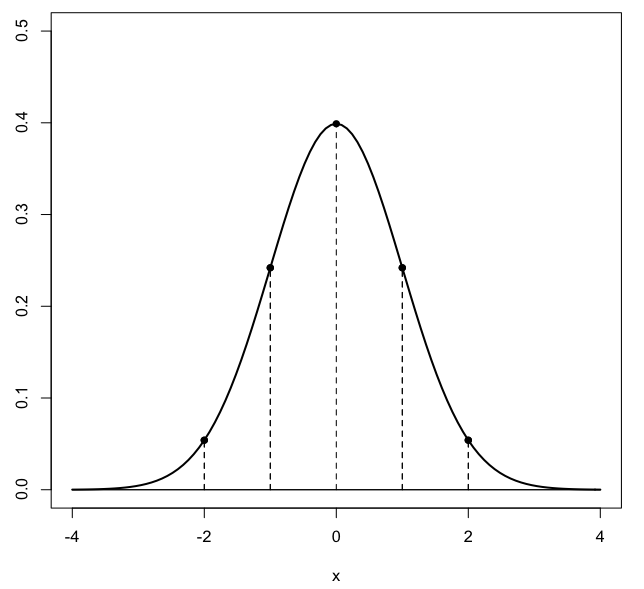
\includegraphics [scale=0.4] {gauss3.png} \end{center}

\title{Field of a dipole}
\date{}

\begin{document}
\maketitle
\Large
Consider a dipole with charge $+q$ on one end, at $(a,0)$, and charge $-q$ on the other end $(-a,0)$.  We want to calculate the field due to the dipole at various points in the $xy$-plane.  That gives us everything, since every other plane formed by rotation of this one around the $x$-axis has the same field.  

This material comes from volume II of Shankar's Physics.  The second part, using the potential, has the calculus.  The first part, using the field, is there for contrast and because he uses various tricks to approximate and simplify the answer.

The relevant equation is a variation on Coulomb's Law:
\[ \mathbf{E} = \frac{q}{4 \pi \epsilon_o} \cdot \frac{1}{r^2} \cdot \hat{\mathbf{e_r}} \]

\subsection*{starting with the field, E}

For a general point $(x,y)$ the vector from the positive pole to the point is
\[ (x - a) \hat{\mathbf{i}} + y \hat{\mathbf{j}} \]
the squared distance is
\[ (x - a)^2 + y^2 \]
the unit vector is
\[ \frac{(x - a) \hat{\mathbf{i}} + y \hat{\mathbf{j}}}{((x - a)^2 + y^2)^{1/2}} \]
so
\[ \mathbf{E}_+ = \frac{q}{4 \pi \epsilon_o} \cdot  \frac{ (x - a) \hat{\mathbf{i}} + y \hat{\mathbf{j}} }{((x - a)^2 + y^2)^{3/2}} \]
For the other pole, we get
\[ \mathbf{E}_- = - \frac{q}{4 \pi \epsilon_o} \cdot  \frac{(x + a) \hat{\mathbf{i}} + y \hat{\mathbf{j}}}{((x + a)^2 + y^2)^{3/2}} \]
The total field is the sum of these two.
\[ \mathbf{E} = \frac{q}{4 \pi \epsilon_o} \cdot \ [ \frac{(x - a) \hat{\mathbf{i}} + y \hat{\mathbf{j}} }{((x - a)^2 + y^2)^{3/2}} - \frac{(x + a) \hat{\mathbf{i}} + y \hat{\mathbf{j}} }{((x + a)^2 + y^2)^{3/2}} \ ] \]

\subsection*{special solutions}
On the $x-$axis, $y = 0$ so 
\[ \mathbf{E} = \frac{q}{4 \pi \epsilon_o} \cdot \ [ \frac{(x - a) \hat{\mathbf{i}}  }{(x - a)^3} - \frac{(x + a) \hat{\mathbf{i}} }{(x + a)^3} \ ] \]
\[ = \frac{q}{4 \pi \epsilon_o} \cdot \ [ \frac{(x + a)^2 - (x - a)^2}{(x - a)^2 \ (x + a)^2} \ ] \ \hat{\mathbf{i}} \]
\[ = \frac{q}{4 \pi \epsilon_o} \cdot \ [ \frac{4ax}{(x^2 - a^2)^2} \ ] \ \hat{\mathbf{i}} \]

Define the \textbf{dipole moment} as
\[ \mathbf{p} = 2aq \ \hat{\mathbf{i}} \]
so
\[ \mathbf{E} = \frac{\mathbf{p}}{4 \pi \epsilon_o} \cdot \frac{2x}{(x^2 - a^2)^2}  \]
For $x >> a$ (and since $y=0$, $r = x$):
\[ \mathbf{E} = \frac{1}{2 \pi \epsilon_o} \cdot \frac{\mathbf{p}}{r^3}  \]

On the $y-$axis, $x = 0$ so 
\[ \mathbf{E} = \frac{q}{4 \pi \epsilon_o} \cdot \ [ \frac{(- a) \hat{\mathbf{i}} + y \hat{\mathbf{j}} }{((- a)^2 + y^2)^{3/2}} - \frac{a \hat{\mathbf{i}} + y \hat{\mathbf{j}} }{((a)^2 + y^2)^{3/2}} \ ] \]
\[ = \frac{q}{4 \pi \epsilon_o} \cdot \ [ \frac{2 (- a \hat{\mathbf{i}}) }{(a^2 + y^2)^{3/2}}  \ ] \]
\[ = - \frac{1}{4 \pi \epsilon_o} \cdot \ \frac{\mathbf{p}}{(a^2 + y^2)^{3/2}}   \]
For $y >> a$
\[ \mathbf{E} = - \frac{1}{4 \pi \epsilon_o} \cdot \ \frac{\mathbf{p}}{r^3}  \]
Compare with the $x$-axis:
\[ \mathbf{E} = \frac{1}{2 \pi \epsilon_o} \cdot \frac{\mathbf{p}}{r^3}  \]

In both cases, the field falls like $1/r^3$, but numerically it is twice as large along the $x$-axis for a given $r$.  Also, along the $x$-axis the field points to the right, while along the $y$-axis it points to the left.

\subsection*{general solution}
Shankar does some slick thinking to simplify the general case.  We have a complicated beast:

\[ \mathbf{E} = \frac{q}{4 \pi \epsilon_o} \cdot \ [ \ \frac{ (x - a) \hat{\mathbf{i}} + y \hat{\mathbf{j}} }{((x - a)^2 + y^2)^{3/2}} - \frac{(x + a) \hat{\mathbf{i}} + y \hat{\mathbf{j}}}{((x + a)^2 + y^2)^{3/2}} \ ] \]

Shankar says "$\mathbf{E}$ vanishes when $a = 0$.  The net field is non-zero only becauase $a \ne 0$, and the non-zero part will start out as the first power of $a$ in a Taylor series expansion.  To keep the dimension of the field the same, the extra a must really be $a/r$", and we saw that in the simple cases above because we had an extra $\mathbf{p}/r$ and $\mathbf{p}$ is proportional to $a$.

Then:  (the equation) has two parts, each with a numerator divided by the denominator, or the numerator times the inverse denominator. We can get the single power of $a$ from either term, and the $a_0$ term from the other.  If we get $a^1$ from the numerator we may set $a = 0$ in the denominator and vice-versa.

Consider 
\[ \mathbf{E}_+ = \frac{q}{4 \pi \epsilon_o} \cdot  \frac{(x - a) \hat{\mathbf{i}} + y \hat{\mathbf{j}}}{((x - a)^2 + y^2)^{3/2}} \]
\[ = \frac{q}{4 \pi \epsilon_o} \cdot  \frac{\mathbf{r} - a \hat{\mathbf{i}} }{((x - a)^2 + y^2)^{3/2}} \]
\[ = \frac{q}{4 \pi \epsilon_o} \cdot \ [ \  \frac{\mathbf{r} }{((x - a)^2 + y^2)^{3/2}} - \frac{a \hat{\mathbf{i}}}{((x - a)^2 + y^2)^{3/2}} \ ] \]
Expand
\[ = \frac{q}{4 \pi \epsilon_o} \cdot \ [ \  \frac{\mathbf{r} }{((x^2 - 2ax + a^2 + y^2)^{3/2}} - \frac{a \hat{\mathbf{i}}}{((x^2 - 2ax + a^2 + y^2)^{3/2}} \ ] \]
\[ \approx \frac{q}{4 \pi \epsilon_o} \cdot \ [ \  \frac{\mathbf{r} }{((x^2 - 2ax + y^2)^{3/2}} - \frac{a \hat{\mathbf{i}}}{((x^2 + y^2)^{3/2}} \ ] \]

In the first term, we keep $\mathbf{r}$ on top (which is $a^0$), so we keep $a^1$ but not $a^2$ on the bottom.   In the second term, we keep $a^1$ on top, so we don't need to keep any terms involving $a$ on the bottom.  Now substitute $r^2 = x^2 + y^2$:

\[ \mathbf{E}_+ \approx \frac{q}{4 \pi \epsilon_o} \cdot \ [ \  \frac{\mathbf{r} }{(r^2 - 2ax)^{3/2}} - \frac{a \hat{\mathbf{i}}}{r^3} \ ] \]

In dealing with $\mathbf{E}_-$, we change the sign on both $q$ and $a$

\[ \mathbf{E}_- \approx - \frac{q}{4 \pi \epsilon_o} \cdot \ [ \  \frac{\mathbf{r} }{(r^2 + 2ax)^{3/2}} + \frac{a \hat{\mathbf{i}}}{r^3} \ ] \]

so the total field due to the dipole is

\[ \mathbf{E} \approx \frac{q}{4 \pi \epsilon_o} \cdot \ [ \  \frac{\mathbf{r} }{(r^2 - 2ax)^{3/2}} -  \frac{\mathbf{r} }{(r^2 + 2ax)^{3/2}} - 2 \frac{a \hat{\mathbf{i}}}{r^3} \ ] \]

Then, bringing out $1/r^3$
\[ \approx \frac{q}{4 \pi \epsilon_o r^3} \cdot \ [ \  \frac{\mathbf{r} }{(1 - 2ax/r^2)^{3/2}} -  \frac{\mathbf{r} }{(1 + 2ax/r^2)^{3/2}} - 2 a \hat{\mathbf{i}} \ ] \]

A last simplification comes from $(1 + z)^n = 1 + nz + \dots$
\[ (1 - 2ax/r^2)^{-3/2} = 1 - \frac{-3}{2} \ \frac{2ax}{r^2} \]
\[ = 1 +  \frac{3ax}{r^2} \]
Hence
\[ \mathbf{E} \approx \frac{q}{4 \pi \epsilon_o r^3} \cdot \ [ \ - 2 a \hat{\mathbf{i}} + \mathbf{r} (1 + \frac{3ax}{r^2}) - \mathbf{r} (1 - \frac{3ax}{r^2}) \ ] \]
\[ \mathbf{E} \approx \frac{q}{4 \pi \epsilon_o r^3} \cdot \ [ \ - 2 a \hat{\mathbf{i}} + 3 \mathbf{r} \frac{2ax}{r^2} \ ] \]
\[ \approx \frac{1}{4 \pi \epsilon_0 r^3} \ [ \  \ - \mathbf{p} + 3 \mathbf{r} \ \frac{(\mathbf{p} \cdot \mathbf{r} )}{r^2} \ ] \]
since $\mathbf{p} \cdot \mathbf{r} = 2axq$.

\subsection*{starting with the potential, V}

The potential is the integral of the field dotted with $\mathbf{r}$, going to some agreed-upon end point, like $\infty$, with zero potential.  The basic equation is
\[ V = \frac{q}{4 \pi \epsilon_0 r} \]
In this case we add the signed contributions from each pole
\[ V = \frac{q}{4 \pi \epsilon_0} \ [ \frac{1}{r_+} -  \frac{1}{r_-}  \ ] \]
That's it for the potential.

We will simplify by moving things to the numerator like so
\[ V = \frac{q}{4 \pi \epsilon_0} \ [ \frac{r_- - r_+}{r_+ r_-}  \ ] \]

But first, extend this by defining the position vector $\mathbf{r}$ relative to the center of the dipole so that in terms of vectors
\[ \mathbf{r}_+ = \mathbf{r} - a \mathbf{\hat{i}} \]
\[ \mathbf{r}_- = \mathbf{r} + a \mathbf{\hat{i}} \]
and
\[ r_+ = \sqrt{\mathbf{r}_+ \cdot \mathbf{r}_+} \]
\[ = \sqrt{r^2 + a^2 - 2 \mathbf{r} \cdot a \mathbf{\hat{i}}} \]

Approximate (for $r >> a$) by setting $a^2 = 0$ and pulling out $r$:
\[ r_+ = r \sqrt{1 - 2 \mathbf{r} \cdot a \mathbf{\hat{i}}/r^2}  \]
\[ r_- = r \sqrt{1 + 2 \mathbf{r} \cdot a \mathbf{\hat{i}}/r^2}  \]

Simplify using the binomial expansion
\[ r_+  \approx r(1 - \mathbf{r} \cdot a \mathbf{\hat{i}}/r^2) \]
\[ r_-  \approx r(1 + \mathbf{r} \cdot a \mathbf{\hat{i}}/r^2) \]
That numerator will be
\[ r_- - r_+ = r(1 + \mathbf{r} \cdot a \mathbf{\hat{i}}/r^2) - r(1 - \mathbf{r} \cdot a \mathbf{\hat{i}}/r^2) \]
\[ = 2 \mathbf{r} \cdot a \mathbf{\hat{i}}/r \]

So now, going back to
\[ V = \frac{q}{4 \pi \epsilon_0} \ [ \frac{1}{r_+} -  \frac{1}{r_-}  \ ] \]
in the brackets, in the numerator we will have what we got in the line before and in the denominator we have
\[ r_+ r_- = r \sqrt{1 + 2 \mathbf{r} \cdot a \mathbf{\hat{i}}/r^2} \cdot r \sqrt{1 - 2 \mathbf{r} \cdot a \mathbf{\hat{i}}/r^2} \]

Approximating the square roots as just equal to $1$ (since $a << r$), that gives
\[ \approx r^2 \]

which leaves us with
\[ V = \frac{q}{4 \pi \epsilon_0} \ [ \frac{2 \mathbf{r} \cdot a \mathbf{\hat{i}}/r}{r^2}  \ ] \]

The dipole moment is
\[ \mathbf{p} = 2 a q \mathbf{\hat{i}} \]
so
\[ V = \frac{1}{4 \pi \epsilon_0} \ [ \frac{\mathbf{p} \cdot \mathbf{r}}{r^3}  \ ] \]

In terms of $\mathbf{r} = \langle x, y \rangle$
\[ \mathbf{p} \cdot \mathbf{r} = 2 a q \mathbf{\hat{i}} \cdot \mathbf{r} = px \]
and $r^2 = x^2 + y^2$ so
\[ V = \frac{p}{4 \pi \epsilon_0} \ [ \frac{x}{(x^2 + y^2)^{3/2}}  \ ] \]

\subsection*{compute the field}

\[ \mathbf{E} = - \nabla V \]
\[ E_x =  - \frac{p}{4 \pi \epsilon_0} \ \frac{\partial}{\partial x} \ [ \ \frac{x}{(x^2 + y^2)^{3/2}}  \ ] \]

The partial derivative is $(u'v - uv')/v^2$ which is
\[ = \frac{(x^2 + y^2)^{3/2} - x \cdot 3/2 (x^2 + y^2)^{1/2} \cdot 2x}{[(x^2  + y^2)^{3/2}]^2} \]
\[ = \frac{1}{(x^2 + y^2)^{3/2}} - \frac{3x^2}{(x^2+y^2)^{5/2}} \]
\[ = \frac{1}{r^3} - \frac{3}{r^3} \ \frac{x^2}{r^2} \]
so
\[ V = \frac{p}{4 \pi \epsilon_0 r^3} \ (3 \cos^2 \theta - 1 ) \]

Similarly
\[ E_y =  - \frac{p}{4 \pi \epsilon_0} \ \frac{\partial}{\partial y} \ [ \ \frac{x}{(x^2 + y^2)^{3/2}}  \ ] \]

The partial is
\[ (- \frac{3}{2}) x \ \frac{1}{(x^2 + y^2)^{5/2}} \ 2y = \frac{-3xy}{r^5} \]
\[ = - \frac{1}{r^3} \ 3 \sin \theta \cos \theta \]

Combining these results, the field is
\[ \mathbf{E} = \frac{p}{4 \pi \epsilon_0 r^3} (3 \cos^2 \theta \mathbf{\hat{i}} -  \mathbf{\hat{i}} + 3 \sin \theta \cos \theta  \mathbf{\hat{j}} \]
\[ \mathbf{E} = \frac{1}{4 \pi \epsilon_0 r^3} (3p \cos^2 \theta \mathbf{\hat{i}} -  p\mathbf{\hat{i}} + 3p \sin \theta \cos \theta  \mathbf{\hat{j}} \]

Since 
\[ \mathbf{p} = p  \mathbf{\hat{i}} \]
The middle term is $- \mathbf{p}$. 

The unit vector is
\[  \mathbf{\hat{e}}_r = \cos \theta  \mathbf{\hat{i}} + \sin \theta  \mathbf{\hat{j}} \]
so the other two terms give
\[ 3p \cos \theta ( \cos \theta \mathbf{\hat{i}} + \sin \theta \mathbf{\hat{j}}) \]
\[ = 3p \cos \theta \ \mathbf{\hat{e}}_r \]
\[ = (3 \mathbf{p} \cdot \mathbf{\hat{e}}_r) \ \mathbf{\hat{e}}_r - \mathbf{p} \]

tacking on the part out front we have
\[ \mathbf{E} =  \frac{1}{4 \pi \epsilon_0 r^3} \ [ \ (3 \mathbf{p} \cdot \mathbf{\hat{e}}_r) \ \mathbf{\hat{e}}_r - \mathbf{p} \ ] \]

which matches what we had above at the end of the section on the field

\[ \approx \frac{1}{4 \pi \epsilon_0 r^3} \ [ \  \ - \mathbf{p} + 3 \mathbf{r} \ \frac{(\mathbf{p} \cdot \mathbf{r} )}{r^2} \ ] \]

allowing for the fact that $\mathbf{r}/r = \mathbf{\hat{e}}_r$.


\end{document}